% #########################################################################
% ##                          FITXER: 6_arima.tex                        ##
% ##                Contingut: Capítol de models ARIMA                   ##
% #########################################################################

\documentclass[../main.tex]{subfiles}

% ------------------------------------------------------------
% Paquets específics
% ------------------------------------------------------------
\usepackage{paquets_format}
%\usepackage{almutils}

% ------------------------------------------------------------
% Inici del document
% ------------------------------------------------------------
\begin{document}


% ============================================================
% CAPÍTOL: Models ARIMA
% ============================================================

\chapter{Modelització amb models ARIMA} \label{ch:Models ARIMA}

\section{Aplicació dels models ARIMA}

Els models ARIMA (\textit{Autoregressive Integrated Moving Average}) són una de les eines estadístiques més utilitzades per a l’anàlisi i la predicció de sèries temporals univariants. Es basen en la idea que el valor actual d’una sèrie pot expressar-se com una combinació lineal dels seus valors passats i dels errors de predicció anteriors, un cop eliminades les possibles tendències o estacionalitats de la sèrie. Aquesta combinació permet capturar l’estructura temporal i generar prediccions a curt termini.

Els models ARIMA han estat aplicats amb èxit en nombrosos camps com l’economia, la medicina, la demografia i la meteorologia \parencite{murat2018forecasting, elseidi2024hybrid}. En el cas concret de la temperatura, diversos estudis han mostrat que poden oferir una línia base sòlida per a la predicció a curt termini, especialment en contextos amb estacionalitat clara o tendències suaus \parencite{tugal2023analysis, koccak2023time}. 

Tot i això, els models ARIMA presenten certes limitacions que cal tenir en compte. D’una banda, tenen diversos punts forts: són estadísticament robustos, fàcilment interpretables i computacionalment eficients, cosa que els fa molt adequats per a prediccions ràpides o contextos on es disposa de recursos limitats. A més, són especialment útils com a línia base per comparar amb models més sofisticats, ja que proporcionen un referent simple però sòlid.

Tanmateix, també tenen limitacions conegudes. Per una banda, assumeixen que les relacions entre els valors passats i futurs de la sèrie són lineals, i que aquesta és estacionària, cosa que pot limitar-ne l’aplicabilitat en casos amb dinàmiques no estacionàries o fortament no lineals. A més, els models ARIMA no permeten incorporar fàcilment informació exògena, com altres variables meteorològiques, a menys que s’utilitzin variants com els models ARIMAX. Finalment, també poden mostrar dificultats en presència de sorolls o anomalies, i tendeixen a perdre precisió en situacions amb canvis sobtats o no previsibles.

Tot i ser una eina senzilla, els models ARIMA i SARIMA ofereixen una base sòlida per a la predicció de sèries temporals, especialment quan es disposa de dades amb estacionalitat i tendències clares. Per aquest motiu, sovint s’utilitzen com a punt de partida en estudis on també es proven models més avançats, com les xarxes neuronals LSTM, servint com a referència per valorar la millora que aporten aquests enfocaments més complexos \parencite{tugal2023analysis, de2020comparison}.



\section{Fonaments dels models ARIMA}

Els models ARIMA van ser proposats originalment per \textcite{box_jenkins} i combinen tres components diferenciats: autoregressiu (AR), integrat (I) i de mitjana mòbil (MA), que permeten capturar la dependència temporal, eliminar tendències i modelitzar la influència d’errors passats.

Un model ARIMA$(p,d,q)$ combina:

\begin{itemize}
    \item Un component autoregressiu d’ordre $p$ (AR), que considera els valors passats de la pròpia sèrie.
    \item Una diferenciació d’ordre $d$ (I), que transforma la sèrie per fer-la estacionària.
    \item Un component de mitjana mòbil d’ordre $q$ (MA), que incorpora els errors de predicció anteriors.
\end{itemize}

La forma general del model és:

\begin{equation}
y_t = c + \sum_{i=1}^{p} \phi_i y_{t-i} + \sum_{j=1}^{q} \theta_j \varepsilon_{t-j} + \varepsilon_t
\label{eq:arima_general}
\end{equation}

on $y_t$ representa el valor observat de la sèrie temporal en el temps $t$, $c$ és una constant (terme independent), i $\phi_i$ i $\theta_j$ són, respectivament, els coeficients dels components autoregressiu (AR) i de mitjana mòbil (MA). Els valors $y_{t-i}$ corresponen als valors passats de la sèrie que intervenen en la part autoregressiva, mentre que els termes $\varepsilon_{t-j}$ són els errors de predicció comesos en instants anteriors, és a dir, la diferència entre el valor observat i el valor predit pel model en aquell moment. Finalment, $\varepsilon_t$ representa el soroll blanc, una seqüència d’errors aleatoris, independents i amb mitjana zero que modelitza la part imprevisible del sistema.


\subsection{Identificació dels paràmetres del model}

Per ajustar un model ARIMA$(p,d,q)$ cal determinar tres paràmetres: $p$ (ordre autoregressiu), $d$ (nombre de diferenciacions) i $q$ (ordre de la mitjana mòbil). Aquest procés de selecció s’inicia habitualment amb la detecció de no estacionarietat, seguida per l’anàlisi de la dependència temporal mitjançant autocorrelacions i, finalment, la comparació entre models amb criteris estadístics.

\vspace{0.5em}
\noindent\textbf{Estacionarietat i diferenciació.}  
Els models ARIMA assumeixen que la sèrie temporal és estacionària, és a dir, que les seves propietats estadístiques, com la mitjana, la variància o l’autocorrelació,es mantenen estables en el temps. Aquesta condició no es compleix sovint en dades reals, especialment en sèries meteorològiques com la temperatura, que presenten tendències i estacionalitats \parencite{de2020comparison}.

Per tal de fer la sèrie estacionària, s’aplica una operació de diferenciació:
\begin{equation}
y'_t = y_t - y_{t-1}
\end{equation}

Aquest procés es pot repetir (diferenciació d’ordre $d$) fins que la sèrie resulti aparentment estacionària. El valor de $d$ és, doncs, un dels paràmetres fonamentals del model. L’estacionarietat es pot verificar amb tests com l’ADF (Augmented Dickey-Fuller), que permeten determinar la necessitat de diferenciació \parencite{koccak2023time}.

\vspace{0.5em}
\noindent\textbf{Determinació de $p$ i $q$.}  
Els paràmetres $p$ i $q$, que defineixen respectivament l’ordre dels components autoregressiu AR (nombre de valors anteriors de la sèrie que s’utilitzen per fer la predicció) i de mitjana mòbil MA (nombre d’errors anteriors que es tenen en compte per corregir la predicció), es poden temptejar mitjançant mètodes gràfics i estadístics.

Gràficament, es pot representar d’autocorrelació (ACF) i autocorrelació parcial (PACF), el que permet identificar l’estructura temporal de la sèrie: un tall brusc a la PACF pot indicar la presència d’un component AR, mentre que un tall a l’ACF pot suggerir un component MA. 

Estadísticament es pot recòrrer els càlculs de l’AIC (Akaike Information Criterion) i el BIC (Bayesian Information Criterion) són útils per comparar diferents configuracions de models i escollir-ne la més adequada. \parencite{murat2018forecasting}

Tot i això, l’elecció final dels paràmetres sovint requereix una validació empírica basada en l’ajust del model i les seves mètriques d’error, respecte l'observació.


\subsection{Extensió estacional: models SARIMA}

Quan la sèrie presenta una estacionalitat clara (com cicles diürns o estacionals), el model ARIMA pot resultar insuficient. En aquests casos, s’utilitza una extensió anomenada SARIMA (\textit{Seasonal ARIMA}), que afegeix components estacionals:

\begin{equation}
\text{SARIMA}(p,d,q)(P,D,Q)_s
\label{eq:sarima_model}
\end{equation}

on $(P, D, Q)$ són els ordres dels components estacionals, i $s$ representa el període de la repetició (per exemple, $s=24$ per cicles diürns en dades horàries o $s=365$ per dades diàries anuals).

Aquest model combina les diferències estacionals i no estacionals per capturar tant les tendències generals com les oscil·lacions periòdiques. Estudis recents mostren que el model SARIMA pot ser especialment útil en la predicció de temperatura quan la sèrie presenta una doble estacionalitat marcada \parencite{murat2018forecasting, koccak2023time}.

La formulació matemàtica completa és la següent:

\begin{equation}
\Phi_P(B^s) \, \phi_p(B) \, (1 - B)^d (1 - B^s)^D y_t = \Theta_Q(B^s) \, \theta_q(B) \, \varepsilon_t
\label{eq:sarima_expandida}
\end{equation}

El model SARIMA es formula com una combinació dels components estacionals i no estacionals. L’element $B$ representa l’operador de retard , de manera que $B y_t = y_{t-1}$. Els polinomis $\phi_p(B)$ i $\theta_q(B)$ corresponen als components autoregressiu (AR) i de mitjana mòbil (MA) no estacionals, d’ordre $p$ i $q$, respectivament. Els termes estacionals s’expressen mitjançant els polinomis $\Phi_P(B^s)$ i $\Theta_Q(B^s)$, que representen els components autoregressiu i de mitjana mòbil estacionals, amb període $s$ i ordres $P$ i $Q$.

Les transformacions $(1 - B)^d$ i $(1 - B^s)^D$ introdueixen la diferenciació no estacional i estacional, amb l’objectiu de garantir l’estacionarietat de la sèrie a curt i llarg termini. Finalment, $\varepsilon_t$ representa el soroll blanc, és a dir, una seqüència d’errors aleatoris amb mitjana zero i no auto-correlacionats.

Això permet capturar simultàniament les estructures a curt i llarg termini, així com la periodicitat intrínseca de la sèrie. En el cas de dades meteorològiques com la temperatura, resulta útil per modelitzar tant l’evolució diària (per exemple, cicles nit-dia amb $s = 24$) com les variacions estacionals anuals ($s = 365$ en dades diàries).


\section{Plantejament de models}

Tal com s'ha desenvolupat anteriorment, els paràmetres controlables dels models ARIMA són els que es poden observar a la \cref{tab:resum_params_arima}
\begin{table}[H]
    \centering
    \renewcommand{\arraystretch}{1.3}
    \begin{tabular}{lll}
        \toprule
        \textbf{Paràmetre} & \textbf{Valors provats} & \textbf{Tipus} \\
        \midrule
        \texttt{p}, \texttt{q} (ordre AR i MA)   & [2, 4, 6, 10]   & A optimitzar \\
        \texttt{d} (diferenciació)              & 1               & Fixat \\
        \midrule
        \texttt{P}, \texttt{Q} (ordre estacional) & [0, 1, 2]      & A optimitzar (SARIMA) \\
        \texttt{D} (diferenciació estacional)     & 0              & Fixat \\
        \texttt{s} (període estacional)           & 24             & Fixat \\
        \midrule
        \texttt{dies d’entrenament}              & [30, 60, 90]    & A optimitzar \\
        \bottomrule
    \end{tabular}
    \caption{Resum de paràmetres considerats en els experiments amb models ARIMA i SARIMA.}
    \label{tab:resum_params_arima}
\end{table}
Els valors escollits per als paràmetres responen a una combinació de criteris pràctics, intuïcions basades en proves preliminars i referències de la literatura \parencite{elseidi2024hybrid, murat2018forecasting, koccak2023time}. En el cas de $p$ i $q$, s’han considerat valors d’entre 2 i 10 per explorar models des de molt senzills fins a d’altres amb més capacitat de memòria. Tot i que en alguns casos podrien utilitzar-se ordres més alts, això incrementa molt la complexitat del model i el risc de sobre-ajustament, sobretot en finestres d’entrenament curtes. La diferenciació $d = 1$ s’ha fixat, ja que és un valor habitual per eliminar tendències suaus, i en les sèries de temperatura acostuma a ser suficient per assolir l’estacionarietat.

Pel que fa a la component estacional, s’ha optat per mantenir el període fix a $s = 24$ per capturar l’estacionalitat diària pròpia de dades horàries. Es prova l’efecte d’afegir components estacionals ($P$, $Q$) fins a valor 2, però es manté $D = 0$ per simplicitat, ja que la diferenciació no estacional sol ser suficient per eliminar la major part de les tendències i oscil·lacions lentes. Les combinacions estacionals permeten veure si afegir estructura cíclica millora realment la capacitat predictiva del model o si n’hi ha prou amb una formulació ARIMA més senzilla.

Finalment, també s’ha volgut analitzar l’impacte de la quantitat d’historial disponible a l’hora d’entrenar els models, tot variant la mida de la finestra entre 30 i 90 dies. Aquesta variació és especialment rellevant en el context d’aquest projecte, on l'estratègia de predicció serà un esquema de \textit{rolling forecast}, en què el model es re-entrena a un nombre de passos determinat (en aquest cas cada 5 passos), utilitzant la finestra d’entrenament més recent. Aquest enfocament permet adaptar-se millor a canvis en la dinàmica de la sèrie, però també és més exigent en termes computacionals i de robustesa del model.


\begin{table}[H]
    \centering
    \small
    \resizebox{\textwidth}{!}{%
    \begin{tabular}{ccccccccccl}
        \toprule
        \textbf{ID} & \texttt{p} & \texttt{d} & \texttt{q} & \texttt{P} & \texttt{D} & \texttt{Q} & \texttt{s} & \texttt{dies\_ent} & \textbf{Tipus} & \textbf{Notes} \\
        \midrule
        A0 & 2  & 1 & 2  & 0 & 0 & 0 & 24 & 60  & ARIMA & Bàsic sense estacionalitat \\
        A1 & 4  & 1 & 4  & 0 & 0 & 0 & 24 & 60  & ARIMA & Més memòria autoregressiva i MA \\
        A2 & 10 & 1 & 10 & 0 & 0 & 0 & 24 & 60  & ARIMA & Model complex per contrast \\
        A3 & 2  & 1 & 2  & 0 & 0 & 0 & 24 & 30  & ARIMA & Bàsic amb poques dades \\
        A4 & 2  & 1 & 2  & 0 & 0 & 0 & 24 & 90  & ARIMA & Bàsic amb moltes dades \\
        \specialrule{1pt}{1pt}{1pt}
        B0 & 2  & 1 & 2  & 1 & 0 & 1 & 24 & 60  & SARIMA & Amb estacionalitat suau \\
        B1 & 2  & 1 & 2  & 2 & 0 & 2 & 24 & 60  & SARIMA & Estacionalitat més marcada \\
        \specialrule{1pt}{1pt}{1pt}
        C0 & 2  & 1 & 2  & 1 & 0 & 1 & 24 & 30  & SARIMA & Finestra curta, reentrenament constant \\
        C1 & 2  & 1 & 2  & 1 & 0 & 1 & 24 & 60  & SARIMA & Configuració intermèdia \\
        C2 & 2  & 1 & 2  & 1 & 0 & 1 & 24 & 90  & SARIMA & Finestra llarga, més estabilitat \\
        \bottomrule
    \end{tabular}
    }
    \caption{Configuracions experimentals dels models ARIMA i SARIMA amb tots els paràmetres considerats. Es mostren tant les estratègies de predicció directa com les de \textit{rolling forecast}.}
    \label{tab:config_experiments_arima_completa}
\end{table}


\section{Resultats}

La \cref{tab:metrics_arima_sarima} recull les mètriques d’error (RMSE, MSE i MAE) que permeten avaluar els models amb les configuracions provades. En general, els models SARIMA mostren un rendiment superior als ARIMA purs, amb una reducció clara de l’error en tots els indicadors. Aquesta millora es manté consistent fins i tot en escenaris amb diferents longituds de finestra d’entrenament, cosa que reforça la robustesa dels models amb component estacional.

\begin{table}[H]
    \centering
    \small
    \begin{tabular}{lccc}
        \toprule
        \textbf{ID} & \textbf{RMSE} & \textbf{MSE}& \textbf{MAE}\\
        \midrule
        A0 & 1.5372& 2.3631& 1.0516\\
        A1 & 1.4075& 1.9812& 0.9793\\
        A2 & 1.4203& 2.0174& 0.9768\\
        A3 & 1.5351& 2.3565& 1.0499\\
        A4 & 1.5164& 2.2994& 1.0405\\
        \specialrule{1pt}{1pt}{1pt}
        B0 & 1.3145& 1.7279& 0.9371\\
        B1 & 1.3146& 1.7283& 0.9335\\
        \specialrule{1pt}{1pt}{1pt}
        C0 & 1.3243 & 1.7485 & 0.9434 \\
        \textbf{C1} & \textbf{1.3145}& \textbf{1.7279} & \textbf{0.9371} \\
        C2 & 1.3155& 1.7306 & 0.9300 \\
        \bottomrule
    \end{tabular}
    \caption{Resultats de les mètriques d’error obtingudes per a cada configuració experimental.}
    \label{tab:metrics_arima_sarima}
\end{table}


Es pot observar en els experiments de la sèrie \textit{A} com és la influència dels paràmetres i la finestra d'entrenament.  Augmentar l’ordre \textit{(\texttt{p} i \texttt{q})} o l'historial d'entrenament, comporta algunes millores, però aquestes no són gaire significatives i sovint no compensen l’increment de cost computacional. 

Per altra banda, els models SARIMA de les sèries B i C ofereixen resultats més sòlids. Fins i tot amb configuracions estacionals senzilles, com \texttt{(1,0,1)}, el model és capaç d’adaptar-se de manera efectiva al cicle diari de la temperatura, millorant l’ajust global. En aquests casos, la mida de la finestra d’entrenament no té un impacte substancial en el rendiment, fet que permet una certa flexibilitat operativa. Això es reflecteix en el model \texttt{C1} (SARIMA \texttt{(2,1,2)(1,0,1)} amb període 24) (\cref{fig:arima_c1}) que amb només 60 dies d’entrenament assoleix les millors mètriques,  sent flexible i senzill.


\begin{figure}[H]
    \centering
    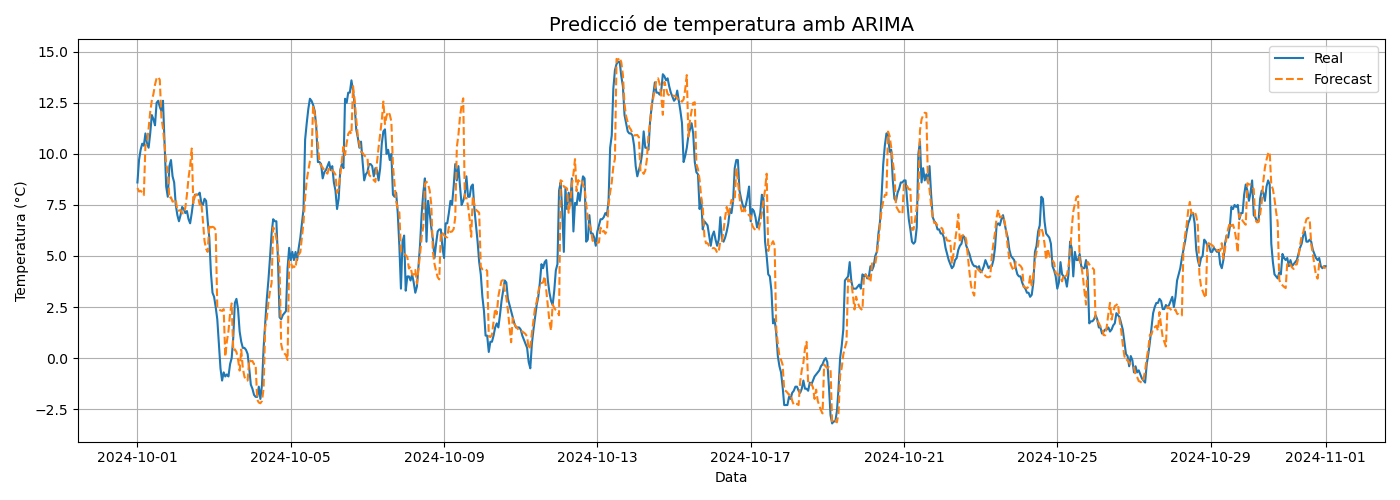
\includegraphics[width=1\linewidth]{figures/arima/C1_plot.png}
    \caption{Visualització de les prediccions del model \texttt{C1} }
    \label{fig:arima_c1}
\end{figure}



% ------------------------------------------------------------
% Fi del document
% ------------------------------------------------------------
\end{document}
